\documentclass[12pt,twoside,a4paper]{report}
\usepackage[a4paper,width=150mm,top=25mm,bottom=25mm,bindingoffset=6mm]{geometry}

\usepackage[utf8x]{inputenc}
\usepackage[slovak]{babel}
\usepackage{palatino,verbatim}

% Balicek pre priamu rec - \say
\usepackage{dirtytalk}

% Balicek "alltt" je to iste ako "verbatim" mod, ale navyse podporuje aj formatovacie znacky textu
\usepackage{alltt}

% Obrazky
\usepackage{graphicx}
\graphicspath{ {obr/} }

% Cislovanie obrazkov a tabuliek
\usepackage{chngcntr}
%Cisluj obrazky nezavisle od cisla kapitol/podkapitol
\counterwithout{figure}{subsection}
\counterwithout{table}{subsection}

% Referencovanie kapitol/sekcii/... podľa ich nadpisu
\usepackage{nameref}

% Tabulky s viacriadkovymi bunkami a zlucenymi bunkami
% Tabulky generujem naastrojom "http://www.tablesgenerator.com/"
\usepackage{booktabs}
\usepackage{multirow}
% LaTeX ma problemy s prikazmi cline a cmidrule, ked je babel nastaveny na slovencinu/cestinu, kvoli definicii pomlcky
% NAMIESTO POMLCKY POUZI ZNAK ZNAMIENKA MINUS "−" (plati hlavne v nazvoch nadpisov a labelov)
\usepackage{etoolbox}
\preto\tabular{\shorthandoff{-}}

%Uloz obrazok tam, kde je deklarovany
%\usepackage[subsection]{placeins}

\newcommand\sktxt[1]{\foreignlanguage{slovak}{#1}}

\begin{document}
\pagenumbering{arabic}

\setcounter{chapter}{1}
\chapter*{MPLS/L3VPN}
\paragraph{}
Andrej Šišila, Marián Vachalík

\tableofcontents

\newpage
\section{Topológia}
\paragraph{}
Budeme konfigurovať smerovacie protokoly MPLS a IS-IS na topológií, ktorá je znázornená na obrázku \ref{fig:mpls_isis_topo}. Vrámci autonómnych systémov sme konfigurovali smerovacie protokoly IS-IS a BGP (iBGP). Medzi autonómnymi systémami sme konfigurovali len BGP (eBGP). IP adresácia je uvedená v tabuľke \ref{tab:ip_adresacia} a dopĺňa grafické znázornenie topológie na obrázku \ref{fig:mpls_isis_topo}. Sieť medzi smerovačmi R1 a R5 nemá mať masku \say{/48} ale \say{/30}.

\begin{figure}[!htbp]
\centering
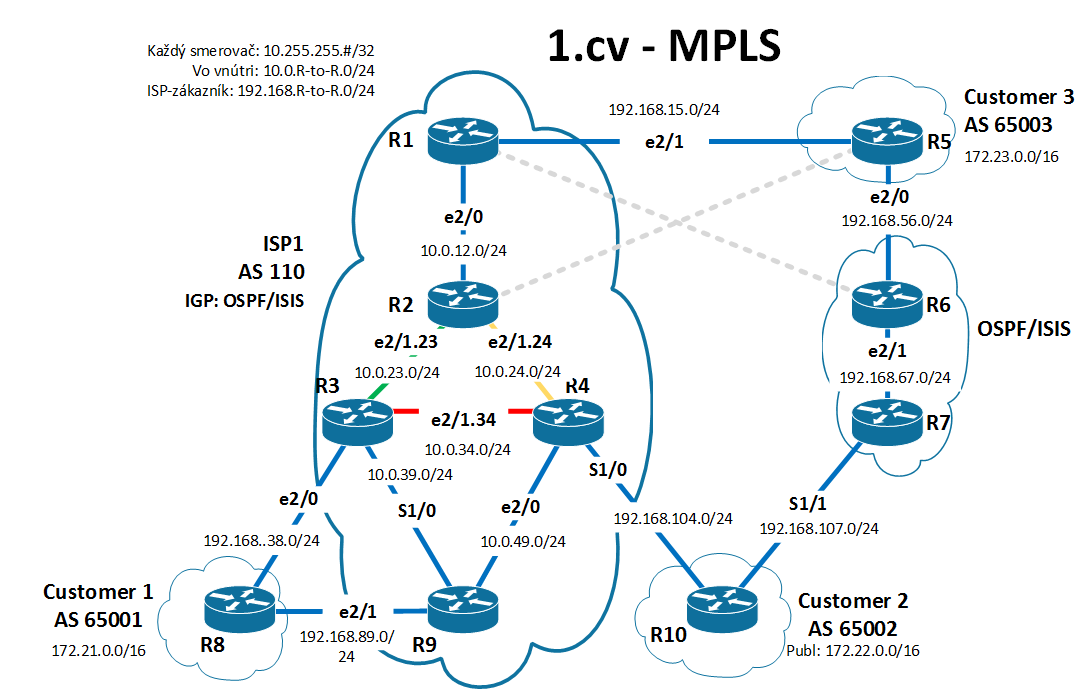
\includegraphics[width=14cm,keepaspectratio]{mpls_isis_topo}
\caption{Topológia MPLS}
\label{fig:mpls_isis_topo}
\end{figure}

\begin{figure}[!htbp]
\centering
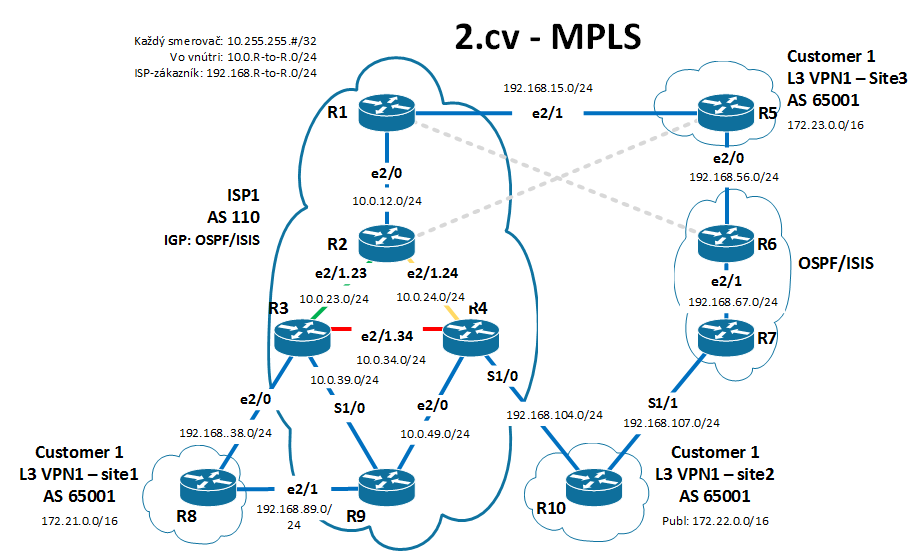
\includegraphics[width=14cm,keepaspectratio]{mpls_l3vpn_topo}
\caption{Topológia MPLS + L3 VPN}
\label{fig:mpls_l3vpn_topo}
\end{figure}



\clearpage


\begin{table}[!htbp]
\centering
\caption{IP adresácia}
\label{tab:ip_adresacia}
\begin{tabular}{|c|l|l|l|}
\hline
\textbf{Smerovač}    & \multicolumn{1}{c|}{\textbf{Rozhranie}} & \multicolumn{1}{c|}{\textbf{IP adresa}} & \multicolumn{1}{c|}{\textbf{Maska}} \\ \hline
\multirow{5}{*}{R1}  & Fa0/0                                   & 200.110.255.249                         & 255.255.255.252                     \\ \cline{2-4} 
                     & Fa0/1                                   & 64.34.255.253                           & 255.255.255.252                     \\ \cline{2-4} 
                     & S1/0                                    & 200.33.255.253                          & 255.255.255.252                     \\ \cline{2-4} 
                     & Lo0                                     & 10.255.255.1                            & 255.255.255.0                       \\ \cline{2-4} 
                     & Lo100                                   & 64.34.1.1                               & 255.255.255.128                     \\ \hline
\multirow{6}{*}{R2}  & Fa0/0                                   & 200.110.255.250                         & 255.255.255.252                     \\ \cline{2-4} 
                     & Fa0/1.23                                & 10.110.23.2                             & 255.255.255.0                       \\ \cline{2-4} 
                     & Fa0/1.24                                & 10.110.24.2                             & 255.255.255.0                       \\ \cline{2-4} 
                     & S1/0                                    & 200.110.255.253                         & 255.255.255.252                     \\ \cline{2-4} 
                     & Lo0                                     & 10.255.255.2                            & 255.255.255.0                       \\ \cline{2-4} 
                     & Lo100                                   & 200.110.0.2                             & 255.255.255.128                     \\ \hline
\multirow{5}{*}{R3}  & Fa0/0                                   & 200.110.255.241                         & 255.255.255.252                     \\ \cline{2-4} 
                     & Fa0/1.23                                & 10.110.23.3                             & 255.255.255.0                       \\ \cline{2-4} 
                     & Fa0/1.34                                & 10.110.34.3                             & 255.255.255.0                       \\ \cline{2-4} 
                     & Lo0                                     & 10.255.255.3                            & 255.255.255.0                       \\ \cline{2-4} 
                     & Lo100                                   & 200.110.0.133                           & 255.255.255.128                     \\ \hline
\multirow{6}{*}{R4}  & Fa0/0                                   & 200.110.255.237                         & 255.255.255.252                     \\ \cline{2-4} 
                     & Fa0/1.24                                & 10.110.24.4                             & 255.255.255.0                       \\ \cline{2-4} 
                     & Fa0/1.34                                & 10.110.34.4                             & 255.255.255.0                       \\ \cline{2-4} 
                     & S1/0                                    & 200.110.255.245                         & 255.255.255.252                     \\ \cline{2-4} 
                     & Lo0                                     & 10.255.255.4                            & 255.255.255.0                       \\ \cline{2-4} 
                     & Lo100                                   & 200.110.1.4                             & 255.255.255.128                     \\ \hline
\multirow{5}{*}{R5}  & Fa0/0                                   & 200.33.255.249                          & 255.255.255.252                     \\ \cline{2-4} 
                     & Fa0/1                                   & 10.100.15.2                             & 255.255.255.252                     \\ \cline{2-4} 
                     & S1/0                                    & 200.110.255.254                         & 255.255.255.252                     \\ \cline{2-4} 
                     & Lo0                                     & 10.255.255.5                            & 255.255.255.0                       \\ \cline{2-4} 
                     & Lo100                                   & 128.45.5.5                              & 255.255.255.128                     \\ \hline
\multirow{5}{*}{R6}  & Fa0/0                                   & 200.33.255.250                          & 255.255.255.252                     \\ \cline{2-4} 
                     & Fa0/1                                   & 10.110.67.6                             & 255.255.255.0                       \\ \cline{2-4} 
                     & S1/0                                    & 200.33.255.254                          & 255.255.255.252                     \\ \cline{2-4} 
                     & Lo0                                     & 10.255.255.6                            & 255.255.255.0                       \\ \cline{2-4} 
                     & Lo100                                   & 200.33.6.6                              & 255.255.255.128                     \\ \hline
\multirow{4}{*}{R7}  & Fa0/1                                   & 10.110.67.7                             & 255.255.255.0                       \\ \cline{2-4} 
                     & S1/1                                    & 200.33.255.245                          & 255.255.255.252                     \\ \cline{2-4} 
                     & Lo0                                     & 10.255.255.7                            & 255.255.255.0                       \\ \cline{2-4} 
                     & Lo100                                   & 200.33.7.7                              & 255.255.255.128                     \\ \hline
\multirow{4}{*}{R8}  & Fa0/0                                   & 200.110.255.242                         & 255.255.255.252                     \\ \cline{2-4} 
                     & Fa0/1                                   & 10.110.89.8                             & 255.255.255.0                       \\ \cline{2-4} 
                     & Lo0                                     & 10.255.255.8                            & 255.255.255.0                       \\ \cline{2-4} 
                     & Lo100                                   & 200.110.12.8                            & 255.255.255.128                     \\ \hline
\multirow{4}{*}{R9}  & Fa0/0                                   & 200.110.255.238                         & 255.255.255.252                     \\ \cline{2-4} 
                     & Fa0/1                                   & 10.110.89.9                             & 255.255.255.0                       \\ \cline{2-4} 
                     & Lo0                                     & 10.255.255.9                            & 255.255.255.0                       \\ \cline{2-4} 
                     & Lo100                                   & 200.110.13.9                            & 255.255.255.128                     \\ \hline
\multirow{4}{*}{R10} & S1/0                                    & 200.110.255.246                         & 255.255.255.252                     \\ \cline{2-4} 
                     & S1/1                                    & 200.33.255.246                          & 255.255.255.252                     \\ \cline{2-4} 
                     & Lo0                                     & 10.255.255.10                           & 255.255.255.0                       \\ \cline{2-4} 
                     & Lo100                                   & 223.255.255.10                          & 255.255.255.128                     \\ \hline
\end{tabular}
\end{table}


% Novu kapitolu davam na novu stranu, lebo bez toho mi zobrazuje tabulku v dalsej kapitole, kde ale tabulka nepatri.
\clearpage

\section{Úlohy}
\subsection{IS-IS}
\subsubsection{Popis}
\paragraph{}

\subsubsection{Konfigurácia}
\paragraph{}

\subsubsection{Overenie}
\paragraph{}








\subsection{MPLS}
\subsubsection{Popis}
\paragraph{}

\subsubsection{Konfigurácia}
\paragraph{}

\subsubsection{Overenie}
\paragraph{}







\subsection{LDP alebo RSVP}
\subsubsection{Popis}
\paragraph{}

\subsubsection{Konfigurácia}
\paragraph{}

\subsubsection{Overenie}
\paragraph{}






\subsection{Router Reflector}
\subsubsection{Popis}
\paragraph{}

\subsubsection{Konfigurácia}
\paragraph{}

\subsubsection{Overenie}
\paragraph{}






\subsection{Multiprotocol BGP}
\subsubsection{Popis}
\paragraph{}

\subsubsection{Konfigurácia}
\paragraph{}

\subsubsection{Overenie}
\paragraph{}





\subsection{Hub \& Spoke VPN}
\subsubsection{Popis}
\paragraph{}

\begin{figure}[!htbp]
\centering
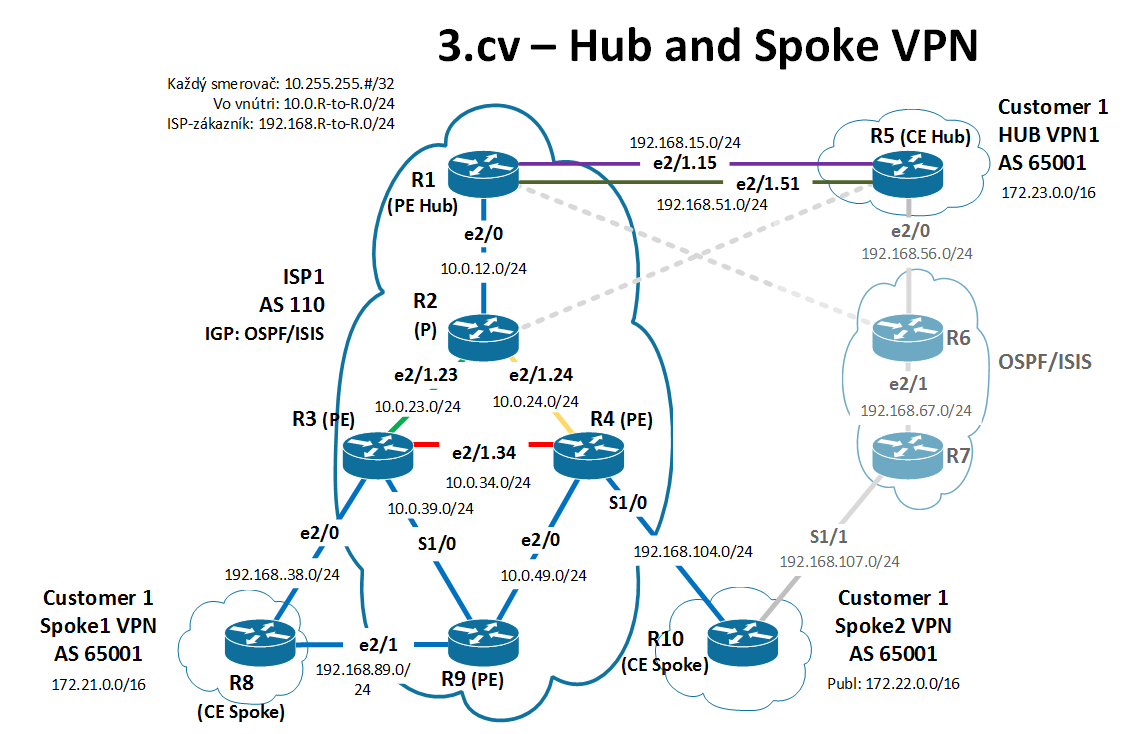
\includegraphics[width=14cm,keepaspectratio]{mpls_hub_spoke_topo}
\caption{Topológia MPLS Hub \& Spoke}
\label{fig:mpls_hub_spoke_topo}
\end{figure}

\begin{figure}[!htbp]
\centering
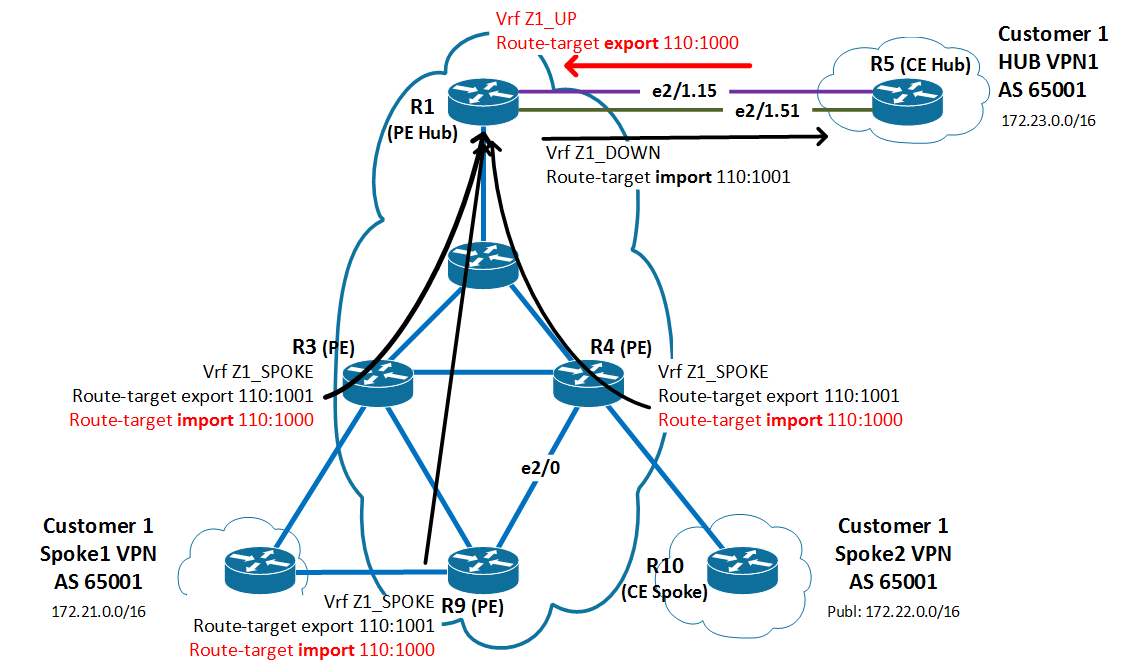
\includegraphics[width=14cm,keepaspectratio]{mpls_hub_spoke_route_target_topo}
\caption{Topológia MPLS Hub \& Spoke s Route Target}
\label{fig:mpls_hub_spoke_route_target_topo}
\end{figure}

\subsubsection{Konfigurácia}
\paragraph{}

\subsubsection{Overenie}
\paragraph{}






\subsection{AS Override}
\subsubsection{Popis}
\paragraph{}

\subsubsection{Konfigurácia}
\paragraph{}

\subsubsection{Overenie}
\paragraph{}






\subsection{MPLS/VPLS}
\subsubsection{Popis}
\paragraph{}

\subsubsection{Konfigurácia}
\paragraph{}

\subsubsection{Overenie}
\paragraph{}



\end{document}